% 第6章第6节：条件数（输入、输出与误差，条件数的定义，基本运算的敏感度）。

\section{条件数}
\label{sec:ls-perturbation}
\label{sec:linear-algebra-stability}
\label{sec:matrix-analysis-conditioning-perturbation}

前五节为线性作用找到了最简形式。从本节起，用这些形式研究线性作用的性质，首先是它对误差的反应。实际交给计算的数据总带误差：测量有噪声，记录有截断，上一步计算有舍入。数据与理想输入相差一点时，答案相差多少？允许范围内的输入增量称为\term{扰动}（perturbation）。扰动分析不改变任务本身，只测量输入的增量在输出中被放大多少倍。

本节先确定怎样度量输入与输出的误差，再定义衡量最坏放大倍数的条件数，说明矩阵的条件数就是最大与最小奇异值之比，最后用同样的增量展开检查几种基本运算。线性方程与最小二乘的解对数据的敏感度，要等第~\ref{chap:linear-equations-and-optimization}章建立求解方法之后，再用本节的工具讨论。

\subsection{输入、输出与误差}

为了统一讨论，把任务看作映射$F$：理想输入$\bm z$对应输出$F(\bm z)$，实际输入为$\bm z+\Delta\bm z$，输出增量为
\[
 \Delta\bm y=F(\bm z+\Delta\bm z)-F(\bm z).
\]
任务不同，比较的输出也不同：矩阵乘向量比较输出向量，求逆比较逆矩阵，解方程比较解向量，谱分解要分别比较特征值与特征子空间。这里只改变数据，不更换算法；算法在机器上产生的舍入误差是另一个来源，第~\ref{chap:linear-equations-and-optimization}章讨论线性方程的数值敏感性时再单独处理。

衡量增量大小有两种方式。\term{绝对误差}（absolute error）直接取增量的范数$\lVert\Delta\bm z\rVert$、$\lVert\Delta\bm y\rVert$。当输入与输出本身有尺度时，更常用\term{相对误差}（relative error）
\[
 \frac{\lVert\Delta\bm z\rVert}{\lVert\bm z\rVert},
 \qquad
 \frac{\lVert\Delta\bm y\rVert}{\lVert F(\bm z)\rVert}.
\]
相对误差在整体缩放下不变，反映变化占原有量的比例；但输出接近零时它失去意义，应改报绝对误差。

误差读数还依赖范数与允许改变的分量：只改右端、同时改矩阵与右端、要求扰动保持对称，是三个不同的扰动问题，敏感度一般不同。

\subsection{条件数的定义}
\label{sec:ls-perturbation-conditioning}

输入增量可以朝任意允许的方向取，敏感度应由最坏方向决定。对足够小的增量，取输出增量与输入增量之比的上确界，
\[
 \kappa_{\mathrm{abs}}(F;\bm z)
 =\lim_{\delta\to0}\ \sup_{0<\lVert\Delta\bm z\rVert\leq\delta}
 \frac{\lVert F(\bm z+\Delta\bm z)-F(\bm z)\rVert}
      {\lVert\Delta\bm z\rVert},
\]
称为任务$F$在$\bm z$处的\term{绝对条件数}（absolute condition number）。对线性作用$\bm x\mapsto\bm A\bm x$，输出增量是$\bm A\Delta\bm x$，增量之比$\lVert\bm A\Delta\bm x\rVert/\lVert\Delta\bm x\rVert$只依赖$\Delta\bm x$的方向，与$\bm x$和$\delta$无关。所以绝对条件数就是第~\ref{sec:ls-matrix-norms}节的诱导范数$\lVert\bm A\rVert$，在最大放大方向达到。

图~\ref{fig:ls-condition-number-amplification}把单位圆与误差圆盘分别送进两个矩阵：良态矩阵的像接近圆，病态矩阵的像被拉成细条，同样半径的误差圆盘反求后沿最弱方向被放大许多倍。

\begin{figure*}[htbp]
 \centering
 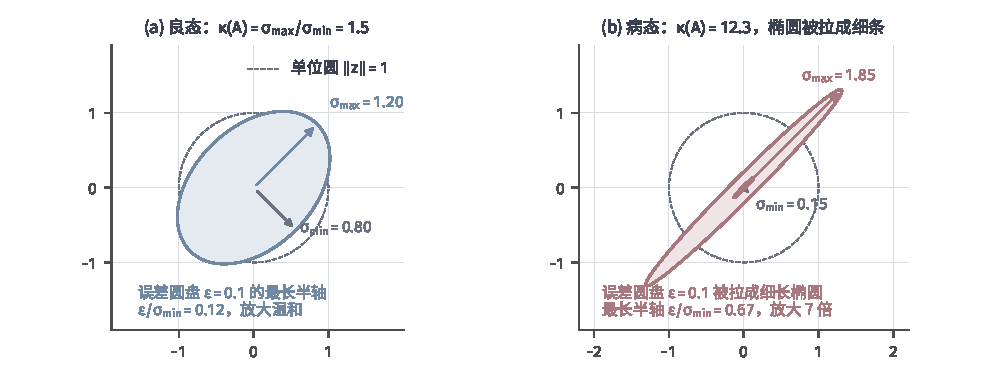
\includegraphics[width=169.0mm]{figures/01-mathematical-preliminaries-upper/02-linear-spaces/matplotlib/ls-condition-number-amplification/ls-condition-number-amplification.pdf}
 \caption{条件数对误差圆盘的放大。灰虚线为单位圆$\lVert\bm z\rVert=1$；左为良态
 $\bm A_1=[[1,0.2],[0.2,1]]$，奇异值$1.20$与$0.80$，$\kappa_2=1.5$，像椭圆接近
 圆；右为病态$\bm A_2=[[1,0.85],[0.85,1]]$，奇异值$1.85$与$0.15$，$\kappa_2\approx12.3$，
 像被拉成细条。半径$\varepsilon=0.1$的误差圆盘（红）最长半轴为$\varepsilon/\sigma_{\min}$：
 良态为$0.125$，病态约$0.67$。}
 \label{fig:ls-condition-number-amplification}
\end{figure*}

把输入、输出都换成相对尺度，得到\term{相对条件数}（relative condition number）
\[
 \kappa_{\mathrm{rel}}(F;\bm z)
 =\lim_{\delta\to0}\ \sup_{0<\lVert\Delta\bm z\rVert\leq\delta}
 \frac{\lVert\Delta\bm y\rVert/\lVert F(\bm z)\rVert}
      {\lVert\Delta\bm z\rVert/\lVert\bm z\rVert}.
\]
对线性作用，$\kappa_{\mathrm{rel}}(\bm A;\bm x)=\lVert\bm A\rVert\lVert\bm x\rVert/\lVert\bm A\bm x\rVert$随$\bm x$变化：$\bm x$落在被压缩的方向上时，输出$\bm A\bm x$小，相对条件数大；落在主伸缩方向上时它小。对可逆方阵再对所有$\bm x$取最坏，令$\bm y=\bm A\bm x$，
\[
 \sup_{\bm x\neq\bm0}\frac{\lVert\bm A\rVert\lVert\bm x\rVert}{\lVert\bm A\bm x\rVert}
 =\lVert\bm A\rVert\sup_{\bm y\neq\bm0}\frac{\lVert\bm A^{-1}\bm y\rVert}{\lVert\bm y\rVert}
 =\lVert\bm A\rVert\,\lVert\bm A^{-1}\rVert ,
\]
这个只依赖矩阵的数就是矩阵的条件数。

\begin{definition}[可逆矩阵的条件数]
\label{def:matrix-analysis-condition-number}
对同一向量范数诱导的矩阵范数，可逆方阵$\bm A$的\term{条件数}（condition number）为
\begin{equation}
 \kappa(\bm A)=\lVert\bm A\rVert\,\lVert\bm A^{-1}\rVert .
 \label{eq:matrix-analysis-condition-number}
\end{equation}
\end{definition}
由第~\ref{sec:ls-svd}节，欧氏范数下$\lVert\bm A\rVert_2=\sigma_{\max}$、$\lVert\bm A^{-1}\rVert_2=1/\sigma_{\min}$，故
\begin{equation}
 \kappa_2(\bm A)=\frac{\sigma_{\max}(\bm A)}{\sigma_{\min}(\bm A)},
 \label{eq:matrix-analysis-spectral-condition-number}
\end{equation}
即最强放大与最弱放大之比。条件数总不小于$1$，因为$1=\lVert\bm I\rVert=\lVert\bm A\bm A^{-1}\rVert\leq\lVert\bm A\rVert\lVert\bm A^{-1}\rVert=\kappa(\bm A)$。正交矩阵的奇异值全为$1$，所以$\kappa_2=1$。矩阵接近奇异时$\sigma_{\min}\to0$，$\kappa_2$增大，与图~\ref{fig:ls-condition-number-amplification}右侧的细长椭圆一致。条件数接近$1$的问题称为良态，条件数很大的问题称为病态。

\begin{theorem}[条件数基本界]
\label{thm:matrix-analysis-condition-number-bound}
设$\kappa(F;\bm z)$为任务$F$在$\bm z$处的相对条件数，则足够小的输入扰动满足
\begin{equation}
 \frac{\lVert\Delta\bm y\rVert}{\lVert F(\bm z)\rVert}
 \lesssim\kappa(F;\bm z)\,\frac{\lVert\Delta\bm z\rVert}{\lVert\bm z\rVert}.
 \label{eq:matrix-analysis-condition-number-bound}
\end{equation}
特别地，可逆系统$\bm A\bm x=\bm b$的右端扰动$\Delta\bm b$引起的解扰动对任意大小的$\Delta\bm b$都满足$\lVert\Delta\bm x\rVert/\lVert\bm x\rVert\leq\kappa(\bm A)\lVert\Delta\bm b\rVert/\lVert\bm b\rVert$。
\end{theorem}
\begin{proof}
第一式是相对条件数定义的直接改写，$\lesssim$表示忽略比$\lVert\Delta\bm z\rVert$高阶的小量。对方程，$\bm A(\bm x+\Delta\bm x)=\bm b+\Delta\bm b$减去$\bm A\bm x=\bm b$，得$\Delta\bm x=\bm A^{-1}\Delta\bm b$，故$\lVert\Delta\bm x\rVert\leq\lVert\bm A^{-1}\rVert\lVert\Delta\bm b\rVert$；又$\lVert\bm b\rVert=\lVert\bm A\bm x\rVert\leq\lVert\bm A\rVert\lVert\bm x\rVert$，即$1/\lVert\bm x\rVert\leq\lVert\bm A\rVert/\lVert\bm b\rVert$。两式相乘即得。
\end{proof}

条件数是最坏方向上的上界，不是每个扰动都达到的倍数。一般任务的相对条件数只控制足够小的扰动；矩阵本身的扰动较大时，还要考虑扰动后是否仍然可逆，这在第~\ref{chap:linear-equations-and-optimization}章估计逆矩阵与方程解的敏感度时处理。

条件数也不回答反复作用的长期结果。下面的反例中，两个矩阵的条件数相同，幂的变化趋势却相反。
\begin{example}[反例：条件数相同而幂的趋势相反]
\label{ex:ls-condition-number-vs-powers}
给定同阶的$2\bm I$与$\tfrac12\bm I$。二者的奇异值分别全为$2$与全为$\tfrac12$，所以
\[
 \kappa_2(2\bm I)=\frac{2}{2}=1,\qquad
 \kappa_2\bigl(\tfrac12\bm I\bigr)=\frac{1/2}{1/2}=1 .
\]
但$(2\bm I)^k=2^k\bm I$逐次增长，$(\tfrac12\bm I)^k=2^{-k}\bm I$逐次衰减。结论：条件数相同的两个矩阵，反复作用的结果可以完全相反。
\end{example}
条件数衡量一次作用的相对放大，长期行为要由谱半径判断（第~\ref{sec:ls-matrix-power-behavior}节），二者不能互相代替。

\subsection{基本运算的敏感度}

同样的增量展开适用于第~\ref{chap:linear-operations}章的基本运算。先看加法。和的增量是$\Delta(\bm x+\bm y)=\Delta\bm x+\Delta\bm y$，由三角不等式，$\lVert\Delta(\bm x+\bm y)\rVert\leq\lVert\Delta\bm x\rVert+\lVert\Delta\bm y\rVert$，所以加法本身不放大绝对误差。但$\bm x\approx-\bm y$时理想输出很小，相对误差被小分母放大，下面的例子给出具体数值。
\begin{example}[加法中的抵消]
\label{ex:ls-cancellation-relative-error}
给定$x=1.0001$、$y=-1.0000$，二者各带至多$5\times10^{-5}$的绝对误差，相对误差约为$5\times10^{-5}$。理想和为$x+y=10^{-4}$，而和的绝对误差至多为$5\times10^{-5}+5\times10^{-5}=10^{-4}$，所以和的相对误差可达
\[
 \frac{10^{-4}}{10^{-4}}=1 .
\]
结论：输入的相对误差约为$5\times10^{-5}$，输出的相对误差却可达$1$，放大约$2\times10^4$倍。
\end{example}
这种抵消不是算法失误，而是问题本身在相对尺度下病态。

再看乘积。它满足
\[
 (\bm A+\bm E)(\bm B+\bm F)-\bm A\bm B=\bm A\bm F+\bm E\bm B+\bm E\bm F,
\]
前两项是一阶响应，各被另一个因子的范数放大，末项在小扰动下是二阶量。

最后看行列式，它在矩阵接近奇异时最敏感。
\begin{example}[接近奇异时的行列式]
\label{ex:ls-determinant-near-singular}
给定$\bm A=\operatorname{diag}(1,\varepsilon)$，$0<\varepsilon<1$，则$\det\bm A=\varepsilon$。把第二个对角元改为$\varepsilon+\delta$，矩阵的相对变化为$\lVert\Delta\bm A\rVert_2/\lVert\bm A\rVert_2=|\delta|$，行列式变为$\varepsilon+\delta$，相对变化为
\[
 \frac{|(\varepsilon+\delta)-\varepsilon|}{\varepsilon}=\frac{|\delta|}{\varepsilon}.
\]
结论：行列式的相对误差是矩阵相对误差的$1/\varepsilon$倍，矩阵越接近奇异，放大越强。
\end{example}

本节得到的结论是：条件数$\kappa(\bm A)=\lVert\bm A\rVert\lVert\bm A^{-1}\rVert$是一次作用下相对误差的最坏放大倍数，欧氏范数下等于$\sigma_{\max}/\sigma_{\min}$，在各方向伸缩悬殊、矩阵接近奇异时变大；加法在抵消时、行列式在矩阵接近奇异时，相对误差也会被小分母放大。这里矩阵始终是固定的，只有输入向量带误差。可是矩阵本身也常常来自数据，例如由有限样本估计的协方差矩阵。下一节把矩阵当作输入，研究它的特征值、奇异值与特征子空间对扰动的敏感度。
